% HMC Math dept HW template example
% v0.04 by Eric J. Malm, 10 Mar 2005
\documentclass[12pt,letterpaper,boxed]{hmcpset}

% set 1-inch margins in the document
\usepackage[margin=1in]{geometry}
\usepackage{alltt}
\usepackage{amsfonts}
\usepackage{amsmath}
\usepackage{amssymb}
\usepackage{amsthm}
\usepackage{booktabs}
\usepackage{caption}
\usepackage{fancyhdr}
\usepackage{graphicx}
\usepackage{mathdots}
\usepackage{mathtools}
\usepackage{microtype}
\usepackage{multirow}
\usepackage{pdflscape}
\usepackage{pgfplots}
\usepackage{siunitx}
\usepackage{slashed}
\usepackage{tabularx}
\usepackage{tikz}
\usepackage{tkz-euclide}
\usepackage[normalem]{ulem}
\usepackage[all]{xy}
\usepackage{imakeidx}
\usepackage{enumerate}
\usepackage{physics}

% include this if you want to import graphics files with /includegraphics
\usepackage{graphicx}

\newcommand{\yy}{y^{(i)}}
\newcommand{\xx}{x^{(i)}}
\renewcommand{\tt}{t^{(i)}}
\newcommand{\ww}{w^{(i)}}
\renewcommand{\ss}{\sigma^{(i)}}
\newcommand{\ind}[1]{\mathbb{I}\{#1\}}
\DeclareMathOperator*{\argmax}{argmax}
\DeclareMathOperator*{\argmin}{argmin}
\newcommand{\thetamap}{\theta_{\mathrm{MAP}}}


% info for header block in upper right hand corner
\name{Runqiu Ye}
\class{Stanford CS299}
\assignment{Problem Set \#2}
\duedate{07/07/2024}

\linespread{1.15}
\begin{document}

\problemlist{Problem Set \#2: Supervised Learning II}

\begin{problem}[Problem 1]
\textbf{Logistic Regression: Training stability}
\end{problem}

\begin{solution}
  \begin{enumerate}[(a)]
    \item The most notable difference in training the logistic regression model on datasets $A$ and $B$ is that the algorithm does not converge on dataset $B$.
    
    \item To investigate why the training procedure behaves unexpectedly on dataset $B$, but not on $A$, we print the value of $\theta$ after every $10000$ iterations. We notice that for data set $B$, although the normalized $\frac{\theta}{\norm{\theta}}$ almost stop changing after several tens of thousands of iterations, each componenet of the unnormalized $\theta$ keeps increasing. We also notice that dataset $A$ is not linearly separable while dataset $B$ is linearly separable.
    
    From the code, we notice that the algorithm calculates the gradient of loss function as 
    \[
    \nabla_{\theta} J(\theta) = -\frac{1}{m} \sum_{i=1}^m \frac{ \yy \xx}{1+ \exp(\yy \theta^T \xx)}.
    \]
    From this, we know that the algorithm uses gradient descent to minimize the loss function
    \[
    J(\theta) = - \frac{1}{m} \sum_{i=1}^m \log \frac{1}{1+ \exp(-\yy \theta^T \xx)}.
    \]

    Hence, for a dataset that is linearly separable, that is, $\yy \theta^T \xx > 0$ for all $i$, a $\theta$ with larger norm always leads to a smaller loss, preventing the algorithm from converging. However, on a dataset that is not linearly separable, there exists $i$ such that $\yy \theta^T \xx < 0$. By plotting $f(z) = \log (1+e^{-z})$ in Figure \ref{fz}, we notice that negative margin dominates when scaling $\theta$ to a larger norm. Hence, we cannot always increase $\theta$ to a larger norm while minimizing $J(\theta)$.

    \begin{figure}
      \centering
      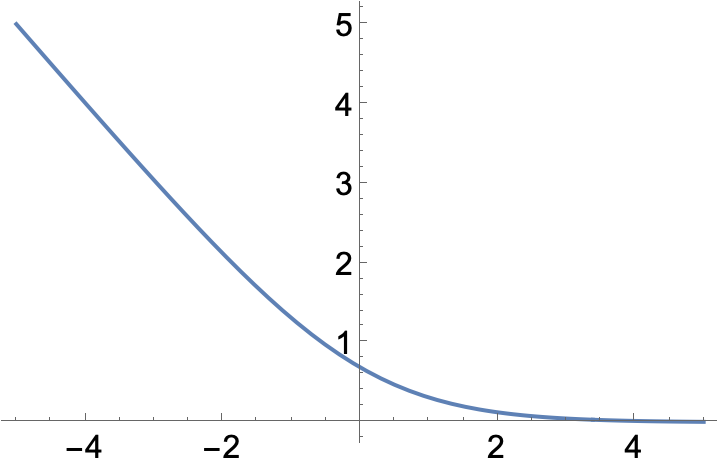
\includegraphics[width=0.6\linewidth]{fz.png}
      \caption{Plot of $f(z) = \log (1+e^{-z})$ for $-5 \leq z \leq 5$.}
      \label{fz}
    \end{figure}
    
    \item Consider the following modifications
    \begin{enumerate}[i.]
      \item Using a different constant learning rate will not make the algorithm converge on dataset $B$, since scaling $\theta$ to larger norm still always decreases the loss.
      \item Decreasing the learning rate over time will make the algorithm converge for dataset $B$, since in this way the change of $\theta$ converge to $0$.
      \item Linear scaling the input features does not help, since it does not change the dataset's linera separability.
      \item Adding a regularization term $\norm{\theta}_2^2$ helps, since now scaling $\theta$ to larger norm penalize the algorithm.
      \item Adding zero-mean Gaussian noise to the training data or labels helps as long as it makes the dataset not linearly separable.
    \end{enumerate}
    
    \item Support vector machines, which uses hinge loss, are not vulnerable to datasets like $B$. In SVM, geometric margin is considered, instead of functional margin considered here. In other words, $\theta$ is normalized, so for linearly separable datasets like $B$, the algorithm will still converge.
  \end{enumerate}
\end{solution}

\begin{problem}[Problem 2]
  \textbf{Model Calibration}

  Try to understand the output $h_\theta (x)$ of the hypothesis function of a logistic regression model, in particular why we might treat the output as a probability.

  When probabilities outputted by a model match empirical observation, the model is \emph{well-calibrated}. For example, if a set of examples $\xx$ for which $h_\theta(\xx) \approx 0.7$, around $70\%$ of those examples should have positive labels. In a well-calibrated model, this property holds true at every probability value. 

  Suppose training set $\{\xx, \yy\}_{i=1}^m$ with $\xx \in \R^{n+1}$ and $\yy \in \{0,1\}$. Assume we have an intercept term $\xx_0 = 1$ for all $i$. Let $\theta$ be the maximum likelihood parameters learned after training logistic regression model. In order for model to be well-calibrated, given any range of probabilities $(a,b)$ such that $0 \leq a < b \leq 1$, and trianing examples $\xx$ where the model outputs $h_\theta (\xx)$ fall in the range $(a,b)$, the fraction of positives in that set of examples should be equal to the average of the model outputs for those examples. That is,
  \[
  \frac{\sum_{i \in I_{a,b}} P(\yy = 1 \mid \xx; \theta)}{\abs{\{i \in I_{a,b}\}}} = \frac{\sum_{i \in I_{a,b}} \ind{\yy = 1}}{\abs{ \{i \in I_{a,b}\} }},
  \]
  where $P(\yy = 1 \mid x; \theta) = h_{\theta} (x) = 1/(1+\exp(-\theta^T x))$, $I_{a,b} = \{i : h_\theta(\xx) \in (a,b) \}$.
\end{problem}

\begin{solution}
  \begin{enumerate}[(a)]
    \item For the described logistic regression model over the range $(a,b) = (0,1)$, we want to show the above equality holds. Recall the gradient of log-likelihood
    \[
    \pdv{\ell}{\theta_j} = \sum_{i=1}^m (\yy - h_{\theta}(\xx)) \xx_j.
    \]
    For a maximum likelihood estimation, $\pdv{\ell}{\theta} = 0$. Hence $\pdv{\ell}{\theta_0} = 0$. Since $\xx_0 = 1$, we have
    \[
    \sum_{i=1}^{m} \yy - h_\theta(\xx) = 0.
    \]
    The desired equality follows immediately since $i \in I_{0,1}$ for all $i$.

    \item A perfectly calibrated model — that is, the equality holds for any $(a,b) \subset [0,1]$ — does not imply that the model achieves perfect accuracy. Consider $(a,b) = (\frac{1}{2}, 1)$, the above equality implies 
    \[
    \frac{\sum_{i \in I_{a,b}} P(\yy = 1 \mid \xx; \theta)}{\abs{\{i \in I_{a,b}\}}} = \frac{\sum_{i \in I_{a,b}} \ind{\yy = 1}}{\abs{ \{i \in I_{a,b}\} }} < 1.
    \]
    This shows that the model does not have perfect accuracy.

    For the converse direction, a perfect accuracy does not imply perfectly calibrated. Consider again $(a,b) = (\frac{1}{2}, 1)$, then we have
    \[
    \frac{\sum_{i \in I_{a,b}} \ind{\yy = 1}}{\abs{ \{i \in I_{a,b}\} }} = 1 > \frac{\sum_{i \in I_{a,b}} P(\yy = 1 \mid \xx; \theta)}{\abs{\{i \in I_{a,b}\}}}.
    \]

    \item Discuss what effect of $L_2$ regularization in the logistic regression objective has on model calibration. For $L_2$ regularization in logistic regression, the gradient becomes
    \[
    \pdv{\ell}{\theta_j} = \sum_{i=1}^m (\yy - h_{\theta}(\xx)) \xx_j - 2C \theta_j = 0.
    \]
    Hence, the equality does not hold unless $\theta_0 = 0$. 
  \end{enumerate}
\end{solution}

\begin{remark}
  The interval $(0,1)$ is the only range for which logistic regression is guaranteed to be calibrated. When GLM assumptions hold, all ranges $(a,b) \subset [0,1]$ are well calibrated. In addition, when test set has same distribution and when model has not overfit or underfit, logistic regression are well-calibrated on test data as well. Thus logistic regression is popular when we are interested in level of uncertainty in the model output. 
\end{remark}

\begin{problem}[Problem 3]
  \textbf{Bayesian Interpretation of Regularization}

  In Bayesian statistics, almost every quantity is a random variable. Joint distribution of all the random variables are called \emph{model} (e.g. $p(x,y,\theta)$). Every unknown quantity can be estimated by conditioning the model on all observed quantities. Such conditional distribution $p(\theta \mid x,y)$ is called \emph{posterior distribution}. A consequence of this approach is that we are required to endow a \emph{prior distribution} $p(\theta)$.

  In purest Bayesian interpretation, we are required to keep the entire posterior distribution over the parameters all the way until prediction to come up with the \emph{posterior predictive distribution}, and the final prediction will be the EV of the posterior predictive distribution. However, this is computationally very expensive.

  The compromise is to estimate a point value of the parameters instead of the full distribution, which is the mode of the posterior distribution. Estimating the mode of posterior distribution is also called \emph{maximum a posteriori estimation} (MAP). That is,
  \[
  \theta_{\mathrm{MAP}} = \argmax_{\theta} p(\theta \mid x,y).
  \]
  Compare this to the \emph{maximum likelihood estimation} (MLE):
  \[
  \theta_{\mathrm{MLE}} = \argmax_{\theta} p(y \mid x, \theta).
  \]

  In this problem, explore connections between MAP estimation and common regularization techniques that are applied with MLE estimation. In particular, we will show how choice of prior distribution over $\theta$ is equivalent to different kinds of regularization.
\end{problem}

\begin{solution}
  \begin{enumerate}[(a)]
    \item Assume that $p(\theta) = p(\theta \mid x)$, we have
    \[
    p(\theta \mid x,y) = \frac{p(y \mid \theta, x)p(\theta \mid x)}{p(y \mid x)} = \frac{p(y \mid \theta, x) p(\theta)}{p(y \mid x)}.
    \]
    Since $p(y \mid x)$ does not depend on $\theta$, 
    \[
    \theta_{\mathrm{MAP}} = \argmax_\theta p(y \mid \theta, x) p(\theta).
    \]
    Note that the assumption $p(\theta) = p(\theta \mid x)$ will be valid for models such as linear regression where the input $x$ are not explicitly modeled by $\theta$. Note also that this means $x$ and $\theta$ are marginally independent, but not conditionally independent when $y$ is given.

    \item Now we show that MAP estimation with a zero-mean Gaussian priori over $\theta$, specifically $\theta \sim \mathcal{N}(0, \eta^2 I)$, is equivalent to applying $L_2$ regularization with MLE estimation. Specifically, we need to show
    \[
    \theta_{\mathrm{MAP}} = \argmin_{\theta} -\log p(y \mid x, \theta) + \lambda \norm{\theta}_2^2.
    \]

    Recall the definition of multivariate normal, we have
    \[
    \begin{aligned}  
      \theta_{\mathrm{MAP}} &= \argmax_\theta p(\theta \mid x,y) \\
      &= \argmax_\theta p(y \mid \theta,x) p(\theta) \\
      &= \argmax_\theta p(y \mid \theta,x) \exp(-\frac{1}{2\eta^2} \norm{\theta}_2^2),
    \end{aligned}
    \]
    where we have ignored some of the constants. Taking the negative log on both sides, it follows that
    \[
    \theta_{\mathrm{MAP}} = \argmin_\theta -\log p(y \mid x, \theta) + \frac{1}{2\eta^2} \norm{\theta}_2^2,
    \]
    as desired, where $\lambda = \frac{1}{2\eta^2}$.

    \item Now consider a specific instance, a linear regression model given by $y = \theta^T x + \epsilon$, where $\epsilon \sim \mathcal{N}(0, \sigma^2)$. Like before, assume a Gaussian prior on this model such that $\theta \sim \mathcal{N}(0,\eta^2 I).$ Let $X$ be the design matrix of all training examples where each row is one example input, and $y$ be the column vector of all the example outputs. We want to derive a closed form expression for $\theta_{\mathrm{MAP}}$.
    
    For this model, the likelihood of an example $(\xx, \yy)$ is
    \[
    p(\yy \mid \xx, \theta) = \frac{1}{\sqrt{2\pi} \sigma} \exp(-\frac{(\yy - \theta^T \xx)^2}{2\sigma^2}).
    \]
    Hence,
    \[
    \log p(\yy \mid \xx, \theta) = - \frac{(\yy - \theta^T \xx)^2}{2\sigma^2} + C,
    \]
    where $C$ is some constant, and $\theta_{\mathrm{MAP}}$ is given by
    \[
    \begin{aligned}
      \theta_{\mathrm{MAP}} &= \argmin_\theta \sum_{i=1}^m \frac{(\yy - \theta^T \xx)^2}{2\sigma^2} + \frac{1}{2\eta^2} \norm{\theta}_2^2 \\
      &= \argmin_\theta \frac{1}{2\sigma^2} (y - X\theta)^T (y - X\theta) + \frac{1}{2\eta^2} \theta^T \theta.
    \end{aligned}
    \]
    Set the gradient of the function to 0, we have
    \[
    0 = -\frac{1}{\sigma^2} X^T(y-X\thetamap) + \frac{1}{\eta^2} \thetamap
    \]
    It follows that
    \[
    \thetamap = \eta^2 (\eta^2 X^T X + \sigma^2 I)^{-1} X^T y.
    \]
    
    \item Now consider the Laplace distribution, whose density 
    \[
    f(z \mid \mu, b) = \frac{1}{2b} \exp(-\frac{\abs{z-\mu}}{b}).
    \]
    As before, consider a linear regression model given by $y = \theta^T x + \epsilon$ where $\epsilon \sim \mathcal{N}(0, \sigma^2)$. Auumer a Laplace prior on this model where $\theta \sim \mathcal{L} (0, bI)$. We want to show that $\thetamap$ in this case is equivalent to the solution of linear regression with $L_1$ regularization, whose loss is specified as
    \[
    J(\theta) = \norm{X\theta - y}_2^2 + \gamma \norm{\theta}_1.
    \]
    
  \end{enumerate}
\end{solution}
\end{document}
